\begin{table}[h]
    \begin{subtable}[h]{0.45\textwidth}
    \begin{tabular}{|c|c|c|}
        \hline
        $m$ (massa) & $l$ (lunghezza) & $k$\\
        \hline

        $(19 \pm 1)\; g$  & $(25.5 \pm 0.5) \;mm$ & $(400 \pm 500)\; Nm^{-1}$\\ 
        $(64 \pm 1)\; g$  & $(27.5 \pm 0.5) \;mm$ & $(250 \pm 70)\; Nm^{-1}$\\ 
        $(91 \pm 1)\; g$  & $(28.5 \pm 0.5) \;mm$ & $(260 \pm 50)\; Nm^{-1}$\\ 
        $(134 \pm 1)\; g$  & $(29.5 \pm 0.5) \;mm$ & $(290 \pm 50)\; Nm^{-1}$\\ 
        $(181 \pm 1)\; g$  & $(31 \pm 0.5) \;mm$ & $(300 \pm 30)\; Nm^{-1}$\\ 
        $(248 \pm 1)\; g$  & $(33 \pm 0.5) \;mm$ & $(300 \pm 30)\; Nm^{-1}$\\ 
        $(387 \pm 1)\; g$  & $(37 \pm 0.5) \;mm$ & $(316 \pm 18)\; Nm^{-1}$\\ 
        $(526 \pm 1)\; g$  & $(41.5 \pm 0.5) \;mm$ & $(313 \pm 13)\; Nm^{-1}$\\ 


        \hline
        
    \end{tabular}
    \end{subtable}
    \hfill
    \begin{subtable}[h]{0.45\textwidth}
        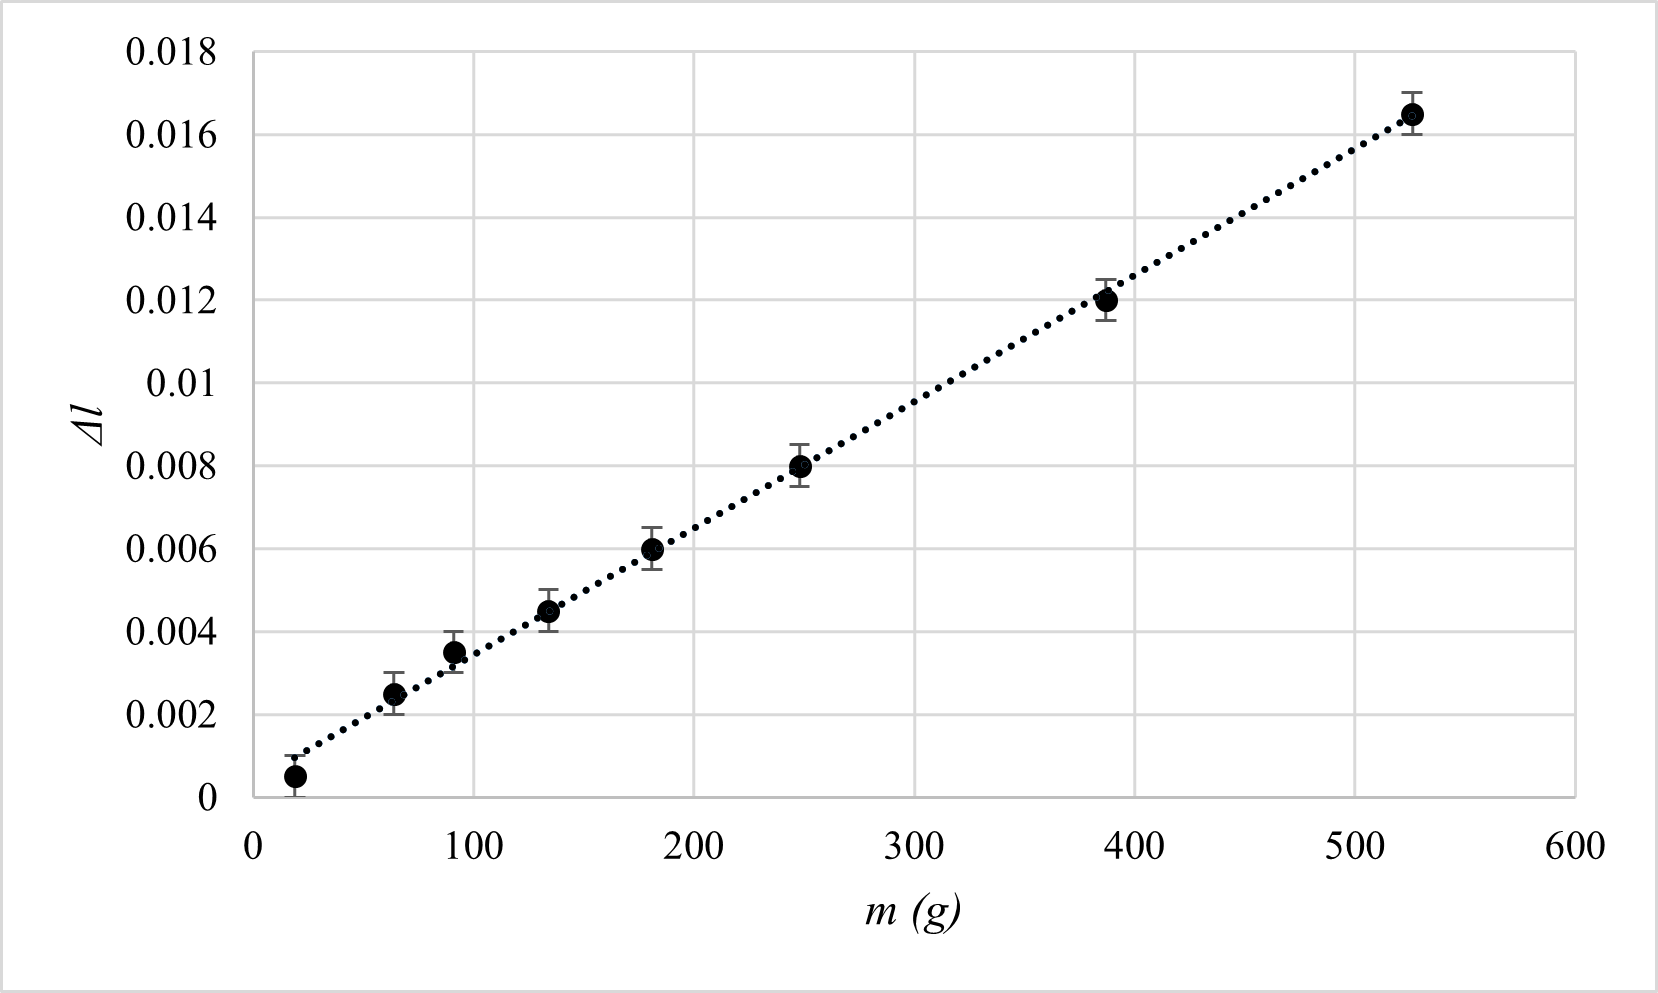
\includegraphics[width = 8cm]{plots/pltMolla.png}
    \end{subtable}
    \caption{Molla ($l_0 = 25.0\, mm \pm 0.5\,mm$) $\qq \sigma_k = 160\; Nm^{-1}$}
    \label{tabellaMolla}
\end{table}
